\documentclass[envcountsame]{llncs}

\usepackage[utf8]{inputenc}
\usepackage{amsmath}
\usepackage{amssymb}
\usepackage{amsfonts}
\usepackage{graphicx}
\usepackage{pdflscape}
\usepackage{algorithm2e}
\usepackage{multicol}
\usepackage{subfig}

\usepackage{bussproofs}
\usepackage{proof}
\usepackage{url}

%\usepackage{pslatex}
\usepackage{fancyvrb}

% Sequent Calculus Proof Settings
\EnableBpAbbreviations
\def\fCenter{\mbox{\ $\vdash$\ }}
\newcommand{\rl}[1]{\RightLabel{#1}}

\usepackage{commands}

\renewcommand{\topfraction}{0.99}	% max fraction of floats at top
\renewcommand{\textfraction}{0.01}	% allow minimal text w. figs
\renewcommand{\floatpagefraction}{0.75}	% require fuller float pages
\renewcommand{\arraystretch}{1.1}


\title{
  Compression of Propositional Resolution Proofs \\
  via Partial Regularization%
  \thanks{This work was partly supported by the ANR DeCert project.}
}

\author{
  Pascal Fontaine%\inst{1}
  \and Stephan Merz%\inst{1}
  \and Bruno Woltzenlogel Paleo%\inst{1}
}

\authorrunning{P.\~Fontaine \and S.\~Merz \and B.\~Woltzenlogel Paleo}

\institute{
  University of Nancy and INRIA, Nancy, France \\
  \{\email{Pascal.Fontaine,Stephan.Merz,Bruno.WoltzenlogelPaleo}\}\email{@inria.fr}
%  \and Technische Universität Wien\thanks{Research carried out while the author was at INRIA Nancy.} \\
%  \email{bruno.wp@gmail.com}
}

% ===========================================================================

\newif\ifcomments
\commentstrue
%\commentsfalse   % gobble comments, set for final version

\ifcomments
  \newcommand{\paf}[1]{\par\noindent{\sf PF: #1}\par\medskip}
  \newcommand{\dd}[1]{\par\noindent{\sf DD: #1}\par\medskip}
  \newcommand{\bw}[1]{\par\noindent{\sf BW: #1}\par\medskip}
  \newcommand{\sm}[1]{\par\noindent{\sf SM: #1}\par\medskip}
  \newcommand{\PAF}[1]{\marginpar{\footnotesize{\sf PF: #1}}}
  \newcommand{\DD}[1]{\marginpar{\footnotesize{\sf DD: #1}}}
  \newcommand{\BW}[1]{\marginpar{\footnotesize{\sf BW: #1}}}
  \newcommand{\SM}[1]{\marginpar{\footnotesize{\sf SM: #1}}}
\else
  \newcommand{\paf}[1]{}
  \newcommand{\dd}[1]{}
  \newcommand{\bw}[1]{}
  \newcommand{\sm}[1]{}
  \newcommand{\PAF}[1]{}
  \newcommand{\DD}[1]{}
  \newcommand{\BW}[1]{}
  \newcommand{\SM}[1]{}
\fi

\newcommand{\RPlong}{\texttt{Recycle\-Pivots}}
\newcommand{\RPIlong}{\texttt{Recycle\-Pivots\-With\-Intersection}}
\newcommand{\LUlong}{\texttt{Lower\-Units}}

\newcommand{\RP}{\texttt{\upshape RP}}
\newcommand{\RPI}{\texttt{\upshape RPI}}
\newcommand{\LU}{\texttt{\upshape LU}}

% ===========================================================================

\begin{document}

\maketitle

\begin{abstract}
This paper describes two algorithms for the compression of propositional
resolution proofs. The first algorithm, \RPIlong, performs partial
regularization, removing an inference $\eta$ when it is redundant in the sense
that its pivot literal already occurs as the pivot of another inference located below in the path from $\eta$ to the root of the proof. The second algorithm, \LUlong, delays the resolution of (both input and derived) unit clauses, thus removing (some) inferences having the same pivot but possibly occurring also in different branches of the proof.

% By generalizing the definition of \emph{regularity}, these two kinds of redundancy, although at first unrelated, can be seen as instances of the same phenomenon.
\end{abstract}


\section{Introduction}

Propositional satisfiability (SAT) solving has made enormous progress
during the recent decade, and powerful decision procedures are being
used in many different contexts, such as hardware and software
verification, knowledge representation, and diagnostic applications
(see~\cite{HandbookOfSAT2009} for a thorough presentation of
techniques and applications of SAT solving). SAT solving also forms
the backbone for automated reasoning over more expressive logics, such
as in SMT (satisfiability modulo theories) solving
(see~\cite{Barrett14} for a detailed account of techniques used in
SMT solvers). For many applications, it is not enough to just obtain a
yes/no answer to the decision problem, but one is also interested in a
justification of the verdict, that is, a model satisfying the original
formula, or a proof showing that no such model exists. For example, in
the context of proof carrying
code~\cite{Necula1997Proof-carrying-code}, the code producer must
provide a proof that will be checked by the code consumer.
% Similarly, when a SAT or SMT solver is integrated as an automated back-end in
% a skeptical proof assistant, the latter requires a proof trace that can be
% verified by its trusted kernel.
In the context of SAT solving, it is well understood how decision
procedures can be adapted to construct a resolution proof while performing proof
search. However, proofs output by SAT solvers can be huge 
(millions of learned clauses and tens or hundreds of
megabytes for typical benchmark cases), and techniques for obtaining small
proofs become of interest. Producing a proof of minimum size is an NP-hard
problem, so it is important to find
heuristics of low (preferably linear) complexity that achieve interesting
reductions in practical cases. Going beyond trivial optimizations, such as
eliminating inferences that do not contribute to the final conclusion, one
frequently observes that the same clause (or the same pivot literal) is used more than once within a proof,
and even along a single branch in a proof. Although it is not a priori the case
that multiple uses of a clause (or pivot) are actually redundant or that their elimination
results in a shorter proof, we concentrate in this work on identifying such
cases and on corresponding transformations of proofs. Our algorithms are
generalizations of similar techniques proposed in the
literature~\cite{Bar-IlanFuhrmannHooryShachamStrichman2009Linear-time-reductions-of-resolution-proofs,Cotton2010Two-Techniques-for-Minimizing-Resolution-Proofs,SimoneBrutomessoSarygina2010An-Efficient-and-Flexible-Approach-to-Resolution-Proof-Reduction}.
We show that our techniques yield provably better results than previous
algorithms, while their implementation is no more complex. A more detailed
comparison with existing work appears in Section~\ref{sec:related}. We have
implemented our algorithms and we presented experimental validations
on standard benchmarks in Section~\ref{sec:evaluation}. 


\section{The Resolution Calculus}

A \emph{literal} is an atomic formula or a negated atomic formula. A
\emph{clause} is a set of literals, $\bot$ denotes the \emph{empty clause}. We
write $\dual{\ell}$ to denote the dual of $\ell$ and $\prop{\ell}$ for the atom
underlying the literal $\ell$
(i.e., $\dual{p} = \neg p$, $\dual{\neg p} = p$, and $\prop{p} = \prop{\neg p} =
p$ for an atomic formula $p$).
%Definition~\ref{definition:Resolution} shows the usual resolution inference rule.

\begin{definition}\label{definition:Resolution}
  A \emph{resolution inference} is an instance of the following rule:
%
  \begin{prooftree}
    \AXC{$\Gamma_1 \cup \{ \ell \} $}
		\AXC{$\Gamma_2 \cup \{ \dual{\ell}  \}$} \RightLabel{$\prop{\ell}$}
    \BIC{$\Gamma_1 \cup \Gamma_2$}
  \end{prooftree}
%
  The clauses $\Gamma_1 \cup \{ \ell \}$ and $\Gamma_2 \cup \{ \dual{\ell}  \}$
  are the inference's \emph{premises} and $\Gamma_1 \cup \Gamma_2$ (the
  \emph{resolvent} of the premises) is its \emph{conclusion}.
  The literal $\ell$ ($\dual{\ell}$) is the \emph{left (right) resolved literal},
  and $\prop{\ell}$ is the \emph{resolved atom} or \emph{pivot}.
%
\hfill\QED
\end{definition}

A \emph{(resolution) proof} of a \emph{clause} $\K$ from a set of
clauses $C$ is a directed acyclic graph (dag): the \emph{input nodes}
are \emph{axiom inferences} (without premises) whose conclusions are elements of
$C$, the \emph{resolvent nodes} are resolution inferences, and the proof has a
node with conclusion $\K$. The dag contains an edge from a node
$\eta_1$ to a node $\eta_2$ if and only if a premise of $\eta_1$ is the conclusion of $\eta_2$. In this case, $\eta_1$ is a \emph{child} of $\eta_2$, and $\eta_2$ is a \emph{parent} of $\eta_1$. A node with no children is a \emph{root}.
A \emph{(resolution) refutation} of $C$ is a resolution proof of $\bot$ from $C$.
For the sake of brevity, given a node $\eta$, we say \emph{clause $\eta$} or 
\emph{$\eta$'s clause} meaning the conclusion clause of $\eta$, 
and \emph{(sub)proof $\eta$} meaning the (sub)proof having $\eta$ as its only root. The resolvent of $\K_1$ and $\K_2$ with pivot $p$ can be denoted as $\K_1
\tRes_p \K_2$. When the pivot is uniquely defined or irrelevant, we omit it and write simply $\K_1 \tRes \K_2$. 
In this way, the set of clauses can be seen as an algebra with a
commutative operator $\tRes$ whose properties have been investigated
in~\cite{FontaineMerzPaleo2010Exploring-and-Exploiting-Algebraic-and-Graphical-Properties-of-Resolution}; 
and terms in the corresponding term algebra denote resolution proofs in a notation style that is more compact
and more convenient for describing resolution proofs than the usual graph notation.

%A clause containing a literal and its dual is called \emph{tautological}. In
%general, two clauses can have more than one resolvent, but then they are all
%tautological. Since resolving a clause $\K$ with a tautological clause always
%results in a resolvent $\K'$ that is \emph{subsumed} by $\K$ (i.e. $\K \subseteq
%\K'$), tautological clauses never contribute for the derivation of $\bot$.
%Therefore, the resolution rule can be modified by forbidding the use of
%tautological clauses as premises or conclusions, and this does not jeopardize
%the refutational completeness of the restricted calculus.
% Furthermore, the
%restricted calculus enjoys uniqueness of resolvents, and thus the unique
%resolvent of two resolvable clauses $\K_1$ and $\K_2$ can be denoted as $\K_1
%\tRes \K_2$. Since the pivot of $\K_1 \tRes \K_2$ is also uniquely defined, it
%is not necessary to mention it explicitly, although we may emphasize it by
%writing, e.g., $\K_1 \tRes_p \K_2$. In this way, clauses form an algebra with a
%commutative operator $\tRes$
%%% SM: was $(\clauses, \tRes)$ -- \clauses not introduced before -- do we need it?
%whose properties have been investigated
%in~\cite{FontaineMerzPaleo2010Exploring-and-Exploiting-Algebraic-and-Graphical-Properties-of-Resolution},
%and terms in the corresponding term-algebra represent resolution proofs compactly
%and conveniently.




\begin{example}
\label{Example:Proof}
Consider the proof $\psi$ shown below:
\vspace{-10pt}
\begin{footnotesize}
\begin{prooftree}
\AXC{$ \eta_1 $}
		\AXC{$ \eta_2: a, c, \neg b $}
				\AXC{$ \eta_1: \neg a$}
						\AXC{$ \eta_3:  a, b $} \RName{$a$}
					\BIC{$ \eta_4: b$} \RName{$b$}
			\BIC{$ \eta_5: a, c$}	\RName{$a$}
	\BIC{$\eta_6: c$}
		\AXC{$ \eta_4 $}
				\AXC{$ \eta_7: a, \neg b, \neg c $} \RName{$b$}
			\BIC{$ \eta_8: a, \neg c$}	\RName{$c$}
					\AXC{$ \eta_1 $}  \RName{$a$}
				\BIC{$ \eta_9: \neg c$}	\RName{$c$}
		\BIC{$\psi: \bot$}	
\end{prooftree}
\end{footnotesize}

The node $\eta_4$ has pivot $a$, left (right) resolved literal $\neg a$ ($a$). Its conclusion is $\{b\}$ and its premises are the conclusions of its parents: the input nodes $\eta_1$ ($\{ \neg a \}$) and $\eta_3$ ($\{ a, b\} $). It has two children ($\eta_5$ and $\eta_8$). $\psi$ can be compactly represented by the following proof term:
$$
(\ub{\{\neg a\}}{\eta_1} \tRes (\{a, c, \neg b\} \tRes \ub{(\eta_1 \tRes \{a, b\})}{\eta_4})) \tRes ((\eta_4 \tRes \{a, \neg b, \neg c\}) \tRes \eta_1).
$$
%
%\hfill\QED   %SM: removed to save some space (and no end marker needed here)
\end{example}



\section{Redundant Proofs}

A proof $\psi$ of $\K$ is considered \emph{redundant} iff there exists another
proof $\psi'$ of $\K'$ such that $\K' \subseteq \K$ (i.e. $\K'$ subsumes $\K$)
and $|\psi'| < |\psi|$ where $|\varphi|$ is the number of nodes in $\varphi$.
The definition below describes two patterns of local redundancy: proofs matching them
 (modulo commutativity of $\tRes$) can be easily compressed.

\begin{definition}[Local Redundancy]\label{def:localredundancy}
  A proof containing a subproof of the shapes (here omitted pivots indicate that the resolvents must be uniquely defined)

  \smallskip
  \centerline{\(
    (\eta \tRes \eta_1) \tRes (\eta \tRes \eta_2)
    \ \quad\text{or}\quad \
    \eta \tRes (\eta_1 \tRes (\eta \tRes \eta_2))
  \)}

  \smallskip\noindent%
  is \emph{locally redundant}.
  Indeed, both of these subproofs can be equivalently replaced by the
  shorter subproof $\eta \tRes (\eta_1 \tRes \eta_2)$.
%
\hfill\QED
\end{definition}

\begin{example}
\label{Example:LocalRedundancies}
The proofs below are two of the simplest examples of locally redundant proofs.
% While $\p{\psi_1}$ exhibits local redundancy of type 1, $\p{\psi_2}$ exhibits local redundancy of type 2.

\vspace{-10pt}
\begin{footnotesize}
\begin{prooftree}
\AXC{$ \eta: \neg a $}
		\AXC{$\eta_1: a, b$} \RName{$\hA{a}$}
	\BIC{$b$}
				\AXC{$\eta$}	
						\AXC{$\eta_2: a, \neg b $} \RName{$\hA{a}$}
					\BIC{$\neg b$} \RName{$b$}
			\BIC{$\psi_1: \bot$}	
\end{prooftree}
\vspace{-10pt}
\begin{prooftree}
\AXC{$\eta: \neg a$}	
		\AXC{$\eta_1: a, b$}
				\AXC{$ \eta $}
						\AXC{$\eta_2: a, \neg b $} \RName{$\hA{a}$}	 
					\BIC{$\neg b$} \RName{$b$} 		
			\BIC{$a$} \RName{$\hA{a}$} 
	\BIC{$\psi_2: \bot$}	
\end{prooftree}
\end{footnotesize}
%
Both proofs can be rewritten to the shorter proof below:

\vspace{-10pt}
\begin{footnotesize}
\begin{prooftree}
\AXC{$\eta: \neg a$}	
		\AXC{$\eta_1: a, b$}
						\AXC{$\eta_2: a, \neg b $} \RName{$b$} 		
			\BIC{$a$} \RName{$\hA{a}$}
	\BIC{$\psi_3: \bot$}	
\end{prooftree}
\end{footnotesize}

Note that, by locally permuting the lowermost inference with pivot $a$ and the
inference with pivot $b$, the proof $\psi_2$ can be transformed into $\psi_1$.
This indicates that the two patterns given in Def.~\ref{def:localredundancy} can
be seen as different manifestations of the same underlying phenomenon. They
appear differently in resolution proofs because the resolution calculus enforces
a sequential order of inferences even when the order actually does not matter.
%
\hfill\QED
\end{example}

In the case of local redundancy, the pairs of redundant inferences having the
same pivot occur close to each other in the proof. However, redundant inferences
can also occur far apart in the proof. One could attempt to remove global
redundancies by repeatedly permuting inferences until the redundant inferences
appear next to each other. However this approach is intrinsically inefficient
because many permutations must be considered and intermediate resolvents must be
recomputed after every permutation.

The following definition generalizes Def.~\ref{def:localredundancy} by
considering inferences with the same pivot that occur within different contexts.
We write $\psi[\eta]$ to denote a \emph{proof-context}
$\psi[\_]$ with a single placeholder replaced by the subproof $\eta$.

\begin{definition}[(Global) Redundancy]\label{def:globalredundancy}
  A proof

  \smallskip
  \centerline{\(
    \psi[\psi_1[\eta \tRes_p \eta_1] \tRes \psi_2[\eta \tRes_p \eta_2]]
    \quad\text{or}\quad
    \psi[ \psi_1[\eta \tRes_p (\eta_1 \tRes \psi_2[\eta \tRes_p \eta_2]) ]]
  \)}

  \smallskip\noindent%
  is \emph{potentially (globally) redundant}. 
  Furthermore, it is \emph{(globally) redundant} if it can be rewritten to one of the following shorter proofs:

  \smallskip
  \centerline{\(
    \psi[\eta \tRes_p (\psi_1[\eta_1] \tRes \psi_2[\eta_2])]
    \ \ \text{or}\ \ 
    \eta \tRes_p \psi[\psi_1[\eta_1] \tRes \psi_2[\eta_2]]
    \ \ \text{or}\ \ 
  	\psi[\psi_1[\eta_1] \tRes \psi_2[\eta_2]].
  \)}
%
%\hfill\QED   % SM: again removed because not needed
\end{definition}

\begin{example}\label{ex:globalredundancy}
  Consider the following proof $\psi$.

  \vspace{-5pt}
  \begin{footnotesize}
  \begin{prooftree}
    \AXC{$\eta: p,q$}   \AXC{$\eta_1: \lnot p, r$}
       \RName{$\hA{p}$}
       \BIC{$q,r$}    \AXC{$\eta_3: \lnot q$}
          \RName{$q$}
          \BIC{$r$}
                              \AXC{$\eta$}   \AXC{$\eta_2: \lnot p, s, \lnot r$}
                                 \RName{$\hA{p}$}
                                 \BIC{$q,s,\lnot r$}    \AXC{$\eta_3$}
                                    \RName{$q$}
                                    \BIC{$s, \lnot r$}
             \RName{$r$}
             \BIC{$\psi: s$}
  \end{prooftree}
  \end{footnotesize}

  It corresponds to the proof term
%
  $((\eta \tRes_{p} \eta_1) \tRes \eta_3) \tRes ((\eta \tRes_{p} \eta_2) \tRes \eta_3)$,
%
  which is an instance of the first pattern appearing in
  Def.~\ref{def:globalredundancy}, hence $\psi$ is potentially globally
  redundant. However, $\psi$ is not globally redundant: the replacement terms
  according to Def.~\ref{def:globalredundancy} contain
%
  $(\eta_1 \tRes \eta_3) \tRes (\eta_2 \tRes \eta_3)$,
%
  which does not correspond to a proof. In particular, neither $\eta_1$ nor
  $\eta_2$ can be resolved with $\eta_3$, as they do not contain the literal
  $q$.
%
\hfill\QED
\end{example}

% As the previous definition suggests, it is not always possible to rewrite an
% potentially globally redundant proof of $\K$ into a shorter proof of $\K'$ with
% $\K' \subseteq \K$. Indeed, $\eta$'s clause may contain a literal
% different from $p$ that is resolved

% The reason for this impossibility is that we may not permute
% the two inferences $\eta \tRes_p [\ ]$ down and outside their proof-contexts
% $\psi_1[\ ]$ and $\psi_2[\ ]$ if $\eta$'s clause contains a literal different
% from $p$ that is resolved within $\psi_1[\ ]$ and $\psi_2[\ ]$, because then
% this literal may not be resolved in the proof-context $\psi[\ ]$ and may appear
% in final clause of the whole proof. This is explained more formally in the proof
% of the following theorem.

% \begin{theorem}
% \label{Theorem:ApparentRedundanciesNotAlwaysRedundancies}
% There are potential global redundancies that are not global redundancies.
% \end{theorem}
% \begin{proof}
% Let $\varphi$ be a proof of a clause $\K$. Let it be potentially globally redundant of type 1 (the proof  for redundancy of type 2 is analogous), and hence of the form $\psi[\psi_1[\eta \tRes_p \eta_1] \tRes \psi_2[\eta \tRes_p \eta_2]]$. Suppose that $\eta$'s clause $C_{\eta}$ is such that $\{p,\ell\} \subseteq C_{\eta}$, where $\ell$ is an atom that is resolved later on within the context $\psi_1[\ ]$. Furthermore, assume that there are no inferences with pivot $\ell$ in the proof-context $\psi[\ ]$ and $\ell \notin \K$. Then, $\psi[\eta \tRes_p (\psi_1[\eta_1] \tRes \psi_2[\eta_2])]$ is a proof of a clause $\K'$ such that $\ell \in \K'$, and hence $\K' \nsubseteq \K$. Consequently, $\varphi$ cannot be rewritten to $\psi[\eta \tRes_p (\psi_1[\eta_1] \tRes \psi_2[\eta_2])]$, and therefore $\varphi$ is not globally redundant with respect to the two inferences with pivot $p$.
% %
% \hfill\QED
% \end{proof}

The second pattern of potentially globally redundant proofs appearing in
Def.~\ref{def:globalredundancy} is related to the well-known notion of
\emph{regularity}~\cite{Tseitin1983On-The-Complexity-of-Proofs-in-Propositional-Logics}. %
Informally, a proof is irregular if there is a path from a node to the root of
the proof such that a literal is used more than once as a pivot in this path. 
%A formal definition using proof-contexts is given below.

\begin{definition}[Irregularity] \label{def:irregularity}
  A proof of the form
%
%  \SM{Removed one context because it's redundant, and irregularity is later used
%    in this form.}
%
  $\psi[ \eta \tRes_p (\eta_1 \tRes \psi'[\eta' \tRes_p \eta_2]) ]$
  is \emph{irregular}.
%
\hfill\QED
\end{definition}

The \emph{regular resolution calculus} is the resolution calculus restricted so that irregular proofs are disallowed. Although it is still complete, it does not p-simulate the unrestricted resolution calculus \cite{Tseitin1983On-The-Complexity-of-Proofs-in-Propositional-Logics}: there are unsatisfiable formulas whose shortest regular resolution refutations are exponentially longer than their shortest unrestricted resolution refutations.

%\sm{It isn't clear if we need any of the following. If we decide to keep it,
%  theorem~\ref{thm:g-regular} could perhaps be turned into a remark.}
%
%By analogy, we can define a notion of irregular proofs based on the first
%pattern of potential global redundancies.
%
%\begin{definition}[General Irregularity]\label{def:g-irregularity}
%  A proof is \emph{generally irregular} if it is irregular or if it is of the form 
%%
%  $\psi[\psi_1[\eta \tRes_p \eta_1] \tRes \psi_2[\eta' \tRes_p \eta_2]]$.
%%
%\hfill\QED
%\end{definition}
%
%Conjecture: 1-regular resolution is complete but does not p-simulate unrestricted resolution.
%
%Why? we can transform 2-irregular refutations into 2-regular refutations that are 1-irregular.
%it should be possible to transform 1-irregular refutations into 1-regular refutations that are 2-irregular.
%
%\begin{theorem}\label{thm:g-regular}
%  Generally regular resolution is incomplete.
%\end{theorem}
%\begin{proof}
%A g-regular resolution should not have two inferences with the same pivot. It is easy to see that this is not possible to achieve when trying to refute, for example, the following clause set: $\{\{p,q\},\{p,\neg q\},\{\neg p,q\},\{\neg p,\neg q\} \}$.
%%
%\hfill\QED
%\end{proof}



\section{Algorithm {\LUlong}}

A closer inspection of Example~\ref{ex:globalredundancy}
% the proof of Theorem \ref{Theorem:ApparentRedundanciesNotAlwaysRedundancies}
shows that it relies on $\eta$'s clause containing two literals: its literal $q$ had to be resolved within the proof-contexts $\psi_1[\_]$ and $\psi_2[\_]$, and hence $\eta$ could not be moved outside the contexts. It is easy to see that a potentially redundant proof is always
redundant in case the redundant node contains a unit clause.

\begin{theorem}
\label{Theorem:UnitApparentRedundanciesAlwaysRedundancies}
Let $\varphi$ be a potentially redundant proof, and $\eta$ be the
redundant node. If $\eta$'s clause is a unit clause, then $\varphi$ is
redundant.
\end{theorem}
\begin{proof}
Consider first a proof of the form $\psi[\psi_1[\eta \tRes \eta_1] \tRes \psi_2[\eta \tRes \eta_2]]$ 
and let $\ell$ be the only literal of $\eta$'s clause.
Then the clause $\psi_1[\eta_1] \tRes \psi_2[\eta_2]$ contains the literal
$\dual{\ell}$. Two cases can be distinguished, depending on whether the literal $\dual{\ell}$ gets propagated to the root of $\psi[\_]$:
\begin{enumerate}
\item In all paths from $\psi_1[\eta_1] \tRes \psi_2[\eta_2]$ to the root of $\psi[\_]$, $\dual{\ell}$ gets resolved out: then, the clause $\psi[\psi_1[\eta_1] \tRes \psi_2[\eta_2]]$ is equal to the clause $\psi[\psi_1[\eta \tRes \eta_1] \tRes \psi_2[\eta \tRes \eta_2]]$, and hence the original proof can be rewritten to $\psi[\psi_1[\eta_1] \tRes \psi_2[\eta_2]]$.
%
\item In some paths from $\psi_1[\eta_1] \tRes \psi_2[\eta_2]$ to the root of $\psi[\_]$, $\dual{\ell}$ does not get resolved out: in this case, the clause of $\psi[\psi_1[\eta_1] \tRes \psi_2[\eta_2]]$ is equal to the clause of $\psi[\psi_1[\eta \tRes \eta_1] \tRes \psi_2[\eta \tRes \eta_2]]$ with the additional literal $\dual{\ell}$. Consequently, the clause $\eta \tRes (\psi[\psi_1[\eta_1] \tRes \psi_2[\eta_2]])$ is equal to the clause $\psi[\psi_1[\eta \tRes \eta_1] \tRes \psi_2[\eta \tRes \eta_2]]$, and hence the original proof can be rewritten to $\eta \tRes (\psi[\psi_1[\eta_1] \tRes \psi_2[\eta_2]])$.
\end{enumerate}
In both cases, since the rewriting to one of the three shorter proofs described in Definition \ref{def:globalredundancy} is possible, the proof is redundant.
The case for potentially redundant proofs of the form $\psi[ \psi_1[\eta \tRes_p (\eta_1 \tRes \psi_2[\eta \tRes_p \eta_2])]]$ is analogous.
%
\hfill\QED
\end{proof}

The {\LUlong} ({\LU}) algorithm targets exactly the class of global redundancy
stemming from multiple resolutions with unit clauses.
% defined in Theorem \ref{Theorem:UnitApparentRedundanciesAlwaysRedundancies}.
The algorithm takes its name from the fact that, when this rewriting is done and
the resulting proof is displayed as a dag, the unit node $\eta$ appears lower
(i.e., closer to the root) than it used to appear in the original proof.

A naive implementation exploiting Theorem
\ref{Theorem:UnitApparentRedundanciesAlwaysRedundancies} would require the proof
to be traversed and fixed after each unit node is lowered. It is possible,
however, to do better by first collecting and removing all the unit nodes in a
single traversal, and afterwards fixing the whole proof in a single second
traversal. Finally, the collected and fixed unit nodes have to be reinserted at
the bottom of the proof (cf. Algorithms~\ref{algo:LU} and~\ref{algo:CollectUnits}).

\DefineVerbatimEnvironment{code}{Verbatim}{fontsize=\small, gobble=2, frame=lines, framesep=2mm, numbers=left, firstnumber=last, commandchars=+\[\], codes={\catcode`$=3\catcode`$=3\catcode`^=7}}

%\newcommand{\function}{\textit{function}}
%\newcommand{\return}{\textit{return}}

\newcommand{\la}{\leftarrow}


\restylealgo{boxed}\linesnumbered
\begin{algorithm}[b]
\caption{\label{algo:LU} \LUlong}
\begin{footnotesize}
\SetLine
\SetKwInOut{Input}{input}\SetKwInOut{Output}{output}
\SetKwData{units}{unitsQueue}
\SetKwData{fixedUnits}{fixedUnitsQueue}

\Input{A proof $\psi$}
\Output{A proof $\psi'$ with no global redundancy with unit redundant node}

\BlankLine

(\units, $\psi_b$) $\la$ collectUnits($\psi$)\;
$\psi_f$ $\la$ fix($\psi_b$)\;
\fixedUnits $\la$ fix(\units)\;
$\psi'$ $\la$ reinsertUnits($\psi_f$, \fixedUnits) \;
\Return {$\psi'$}\;
\end{footnotesize}
\end{algorithm}

%\begin{code}
%  +function lowerUnits(p: Proof): Proof = {
%    val units = collectUnits(p)
%    val roots = p::units
%    val fixedP::fixedUnits = fix(roots)
%    val result = reinsertUnits(fixedP, fixedUnits)
%    +return result
%  }
%\end{code}

Care must be taken with cases when a unit node $\eta'$ occurs above in the subproof 
that derives another unit node $\eta$. In such cases, $\eta$ depends on $\eta'$.
Let $\ell$ be the single literal of the unit clause of $\eta'$. 
Then any occurrence of $\dual{\ell}$ in the subproof above $\eta$ will not be cancelled by 
resolution inferences with $\eta'$ anymore. Consequently,
$\dual{\ell}$ will be propagated downwards when the proof is fixed and will appear in the clause of $\eta$.
Difficulties with such dependencies can be easily avoided if we reinsert the upper unit node $\eta'$ after 
reinserting the unit node $\eta$ (i.e. after reinsertion, $\eta'$ must appear below $\eta$, 
to cancel the extra literal $\dual{\ell}$ from $\eta$'s clause). 
This can be ensured by collecting the unit nodes in a queue during a bottom-up traversal of the proof 
and reinserting them in the order they were queued.

\restylealgo{boxed}\linesnumbered
\begin{algorithm}[t]
\begin{footnotesize}
\SetLine
\SetKwInOut{Input}{input}\SetKwInOut{Output}{output}
\SetKwData{units}{unitsQueue}
\SetKwData{fixedUnits}{fixedUnitsQueue}

\Input{A proof $\psi$}
\Output{A pair containing a queue of all unit nodes (\units) that are used more than once in $\psi$ and a broken proof $\psi_b$}

\BlankLine

$\psi_b$ $\la$ $\psi$\;
traverse $\psi_b$ bottom-up and \ForEach{node $\eta$ in $\psi_b$}{
   \If{$\eta$ is unit and $\eta$ has more than one child}{
        add $\eta$ to \units\;
        remove $\eta$ from $\psi_b$\;
      }
  }
\Return {\upshape (\units, $\psi_b$)}\;
\caption{\label{algo:CollectUnits} \texttt{CollectUnits}}
\end{footnotesize}
\end{algorithm}


%\begin{code}
%  function collectUnits(p: Proof): Queue<Proof> = {
%    val units = new Queue<Proof>
%    traverseBottomUp(p)(n => {
%      if (n.clause.size == 1 && n.children.length > 1) {
%        units.enqueue(n)
%        deletedNodeMarker replaces n // children of n have deletedNodeMarker as a parent from now on
%      }
%      n.freeMemory
%    )
%    return units
%  }
%\end{code}

The algorithm for fixing a proof containing many roots performs a top-down traversal of the proof, recomputing the resolvents and replacing broken nodes (e.g. nodes having \texttt{deletedNodeMarker} as one of their parents) by their surviving parents (e.g. the other parent, in case one parent was \texttt{deletedNodeMarker}).

%\begin{code}
%  function fix(p: Proof) = fix(new Queue(p))
%  function fix(proofRoots: Queue<Proof>): Proof = {
%    val mapOldRootsToNewRoots = new HashMap<Proof,Proof>
%    traverseTopDown('proof deriving proofRoots')(n => {
%      if (n is Input) {
%        if (n.children.length == 0) mapOldRootsToNewRoots.add(n, n)
%      }
%      else if (n is Resolvent) {
%         if (n.left.clause.contains(n.resolvedLiterals.left) && 
%             n.right.clause.contains(n.resolvedLiterals.right)) {
%           n.update
%           if (n.left.children.forall(c => c is marked as fixed)) r.left.freeMemory
%           if (n.right.children.forall(c => c is marked as fixed)) r.right.freeMemory
%           if (n.children.length == 0) mapOldRootsToNewRoots.add(n, n)
%         }
%         else {
%           val survivingParent : Proof =
%             if (n.left == deletedNodeMarker) n.right
%             else if (n.right == deletedNodeMarker) n.left
%             else if (n.left.clause.contains(n.resolvedLiterals.left) && 
%                        !n.right.clause.contains(n.resolvedLiterals.right)) n.right
%             else if (!n.left.clause.contains(n.resolvedLiterals.left) && 
%                        n.right.clause.contains(n.resolvedLiterals.right)) n.left
%             else {
%               if (n.left.length < r.right.length) n.left
%               else n.right
%             }
%           survivingParent replaces n
%           delete(n)
%           if (survivingParent.children.length == 0) mapOldRootsToNewRoots.add(n, survivingParent)
%         }
%      }
%      mark n as fixed
%    }
%    )
%    return proofRoots.map(p => madOldRootsToNewRoots(p))
%  }
%\end{code}

When unit nodes are collected and removed from a proof of a clause $\K$ and the
proof is fixed, the clause $\K'$ in the root node of the new proof is not equal
to $\K$ anymore, but contains (some of) the duals of the literals of the unit
clauses that have been removed from the proof. The reinsertion of unit nodes at
the bottom of the proof resolves $\K'$ with the clauses of (some of) the
collected unit nodes, in order to obtain a proof of $\K$ again.
%

%\begin{code}
%  function reinsertUnits(proof: Proof, units: Queue<Proof>): Proof = {
%    var resultProof = proof
%    while (units != emptyQueue) {
%      val u = units.dequeue
%      if (resultProof.clause contains dual of a literal in u.clause) {
%        resultProof = new Resolvent(u, resultProof)
%      }
%    }
%    return resultProof
%  }
%\end{code}

\restylealgo{boxed}\linesnumbered
\begin{algorithm}[!h]
\begin{footnotesize}
\SetLine
\SetKwInOut{Input}{input}\SetKwInOut{Output}{output}
\SetKwData{units}{q}
\SetKwData{fixedUnits}{fixedUnitsQueue}

\Input{A proof $\psi_f$ (with a single root) and a queue \units of root nodes}
\Output{A proof $\psi'$}

\BlankLine
$\psi'$ $\la$ $\psi_f$\;
    \While{\units $\neq$ $\emptyset$}{
      $\eta$ $\la$ first element of \units \;
      \units $\la$ tail of \units \;
      \If{$\eta$ is resolvable with root of $\psi'$}{
        $\psi'$ $\la$ resolvent of $\eta$ with the root of $\psi'$ \;
      }
    }
\Return {\upshape $\psi'$}\;
\caption{\label{algo:ReinsertUnits} \texttt{ReinsertUnits}}
\end{footnotesize}
\end{algorithm}


\begin{example}
When applied to the proof $\psi$ shown in Example \ref{Example:Proof}, the algorithm {\LU} collects the nodes $\eta_4$ and $\eta_1$, and replaces them by \texttt{deletedNodeMarker} (\texttt{DNM}):

\vspace{-10pt}
\begin{footnotesize}
\begin{prooftree}
\AXC{$ \texttt{DNM} $}
		\AXC{$ \eta_2: a, c, \neg b $}
				\AXC{$ \texttt{DNM} $}
						\AXC{$ \eta_3:  a, b $} \dashedLine \RName{$a$}
					\BIC{$\eta_4: \texttt{DNM}$} \dashedLine \RName{$b$}
			\BIC{$ \eta_5: a, c$}	\dashedLine \RName{$a$}
	\BIC{$\eta_6: c$}
		\AXC{$ \texttt{DNM} $}
				\AXC{$ \eta_7: a, \neg b, \neg c $} \dashedLine \RName{$b$}
			\BIC{$ \eta_8: a, \neg c$}	\RName{$c$}
					\AXC{$ \texttt{DNM} $}  \dashedLine \RName{$a$}
				\BIC{$ \eta_9: \neg c$}	\RName{$c$}
		\BIC{$\psi: \bot$}	
\end{prooftree}
\end{footnotesize}

\noindent Fixing removes the \texttt{DNM}s. The derived unit clause $\eta_4$ is replaced by $\eta_3$, since its other parent was a $\texttt{DNM}$. And the proof $\psi$ becomes:

\begin{footnotesize}
\begin{prooftree}
\AXC{$ \eta_2: a, c, \neg b $}
				\AXC{$ \eta_7: a, \neg b, \neg c $} \RName{$c$}
		\BIC{$\psi: a, \neg b$}	
\end{prooftree}
\end{footnotesize}

\noindent Finally, the collected units $\eta_4$ (now replaced by $\eta_3$) and $\eta_1$ can be reinserted in the bottom of the proof, resulting in $((\eta_2 \tRes \eta_7) \tRes \eta_3) \tRes \eta_1$:

\begin{footnotesize}
\begin{prooftree}
\AXC{$ \eta_2: a, c, \neg b $}
				\AXC{$ \eta_7: a, \neg b, \neg c $} \RName{$c$}
		\BIC{$\psi: a, \neg b$}	
					\AXC{$ \eta_3 (\eta_4):  a, b $}  \RName{$b$}
			 \BIC{$\psi': a$}	
			 			\AXC{$ \eta_1:  \neg a $}  \RName{$a$}
				 \BIC{$\psi'': \bot$}	
\end{prooftree}
\end{footnotesize}
%
\hfill\QED
\end{example}

For efficiency reasons, modern SAT solvers tend to use unit clauses eagerly:
once a unit clause is found, it is used to simplify all other clauses.
While this is clearly a good heuristic during proof search, unit resolutions can
be delayed once a proof is found, since the number of resolution steps can then
be significantly reduced. This effect is illustrated by a toy example in the
proof of Theorem~\ref{Theorem:QuadraticCompression} below. While modern SAT
solvers can produce a linear-size proof for this particular example, it
nevertheless illustrates the undesirable effects that eager unit resolution may
have on proof size.

\begin{theorem}
\label{Theorem:QuadraticCompression}
There is a sequence of unsatisfiable clause sets $S_n$ for which the
shortest refutations $\varphi_n$ obtained via eager unit resolution
grow quadratically (i.e. $|\varphi_n| \in \Omega(n^2)$) while the
compressed proofs $\LU(\varphi_n)$ grow only linearly
(i.e. $|\LU(\varphi_n)| \in O(n)$).
\end{theorem}
\begin{proof} Consider the clause set $S_n$ below:
$$
\K_1 = \neg p_1
\quad
\K_2 = p_1, \neg p_2
\quad
\K_3 = p_1, p_2, \neg p_3
\quad
\ldots
\quad
\K_{n+1} = p_1, p_2, p_3, \ldots, p_n
$$
By \emph{eager unit resolution}, $\K_1$ is firstly resolved with all other $n$ clauses. Then the unit resolvent of $\K_1$ and $\K_2$ is resolved with all resolvents of $\K_1$ and $\K_i$ ($3 \leq i \leq n+1$) and so on\ldots The $k^{th}$ iteration of unit resolution generates $n+1-k$ resolvents. One of these is the unit clause $\K^u_{k+1} = \neg p_{k+1}$ which is then resolved in the next iteration. It is easy to see that this refutation $\varphi_n$ has length
$
\frac{n^2 + n}{2}
$.
The compressed proof $\LU(\varphi_n)$, shown below, has length equal to $n$ only.
$$
(\K_1 \tRes (\ldots \tRes (\K_{n-1} \tRes (\K_n \tRes \K_{n+1}))\ldots))
$$
%
\hfill\QED
\end{proof}


\newcommand{\clause}[1]{#1.\mathit{clause}}

\section{Algorithm {\RPIlong}}
\label{Section:RPI}

Our second algorithm, {\RPIlong} ({\RPI}), aims at compressing irregular proofs. It can be seen as a simple 
but significant modification of the {\RPlong} ({\RP}) algorithm described in 
\cite{Bar-IlanFuhrmannHooryShachamStrichman2009Linear-time-reductions-of-resolution-proofs}, 
from which it derives its name. 
Although in the worst case full regularization can increase the proof length exponentially 
\cite{Tseitin1983On-The-Complexity-of-Proofs-in-Propositional-Logics}, these algorithms show that 
many irregular proofs can have their length decreased if a careful partial regularization is performed. 

Consider an irregular proof of the form $\psi[ \eta \tRes_p \psi'[\eta' \tRes_p \eta''] ]$ and assume, without loss of generality, that $p \in \eta$ and $p \in \eta'$. Then, if $\eta' \tRes_p \eta''$ is replaced by $\eta''$ within the proof-context $\psi'[\ ]$, the clause $\eta \tRes_p \psi'[\eta'']$ subsumes the clause $\eta \tRes_p \psi'[\eta' \tRes_p \eta'']$, because even though the literal $\neg p$ of $\eta''$ is
propagated down, it gets resolved against the literal $p$ of $\eta$ later on below in the proof. More precisely, even though it might be the case that $\neg p \in \psi'[\eta'']$ while $\neg p \notin \psi'[\eta' \tRes_p \eta'']$, it is necessarily the case that $\neg p \notin \eta \tRes_p \psi'[\eta' \tRes_p \eta'']$ and $\neg p \notin \eta \tRes_p \psi'[\eta'']$.

Although the remarks above suggest that it is safe to replace $\eta' \tRes_p
\eta''$ by $\eta''$ within the proof-context $\psi'[\ ]$, this is not always the
case. If a node in $\psi'[\ ]$ has a child in $\psi[\ ]$, then the literal $\neg
p$ might be propagated down to the root of the proof, and hence, the clause
$\psi[ \eta \tRes_p \psi'[ \eta''] ]$ might not subsume the clause $\psi[ \eta
\tRes_p \psi'[\eta' \tRes_p \eta''] ]$. Therefore, it is only safe to do the
replacement if the literal $\neg p$ gets resolved in all paths from $\eta''$ to the root or if it already occurs in the root clause of the original proof $\psi[ \eta \tRes_p \psi'[\eta' \tRes_p \eta''] ]$.

\restylealgo{boxed}\linesnumbered
\begin{algorithm}[!b]
\begin{footnotesize}
\SetLine
\SetKwInOut{Input}{input}\SetKwInOut{Output}{output}
\SetKwData{units}{unitsQueue}
\SetKwData{fixedUnits}{fixedUnitsQueue}

\Input{A proof $\psi$}
\Output{A possibly less-irregular proof $\psi'$}

\BlankLine

$\psi'$ $\la$ $\psi$\;
traverse $\psi'$ bottom-up and \ForEach{node $\eta$ in $\psi'$}{
   % \uIf{$\eta$ is an input node}{ 
   % 		do nothing \;
   %  }
   %  \ElseIf{$\eta$ is a resolvent node}{
   %   setSafeLiterals($\eta$) \;
   %   regularizeIfPossible($\eta$)
   % }
%% SM: original version: do we really need the "do nothing" branch?
   \If{$\eta$ is a resolvent node}{
     setSafeLiterals($\eta$) \;
     regularizeIfPossible($\eta$)
   }
  }
$\psi'$ $\la$ fix($\psi'$) \;
\Return {$\psi'$}\;
\caption{\label{algo:RPI} \texttt{\RPIlong}}
\end{footnotesize}
\end{algorithm}

%\begin{code}
%  function recyclePivotsWithIntersection(p: Proof): Proof = {
%    traverseBottomUp(p)(
%      n => {
%        if (n is Input) doNothing
%        else if (n is Resolvent) {
%          setSafeLiterals(n)
%          regularizeIfPossible(n)
%          for (c in n.children) c.freeMemory
%        } 
%      }
%    )
%    fix(p)  
%  }
%\end{code}

These observations lead to the idea of traversing the proof in a bottom-up
manner, storing for every node a set of \emph{safe literals} that get resolved
in all paths below it in the proof (or that already occurred in the root clause
of the original proof). Moreover, if one of the node's resolved literals belongs
to the set of safe literals, then it is possible to regularize the node by
replacing it by one of its parents (cf.\ Algorithm~\ref{algo:RPI}). 

The regularization of a node should replace a node by one of its parents, and more precisely by the parent whose clause contains the resolved literal that is safe. After regularization, all nodes below the regularized node may have to be fixed. However, since the regularization is done with a bottom-up traversal, and only nodes below the regularized node need to be fixed, it is again possible to postpone fixing and do it with only a single traversal afterwards. 
Therefore, instead of replacing the irregular node by one of its parents immediately, 
its other parent is replaced by \texttt{deletedNodeMarker}, as shown in Algorithm~\ref{algo:Regularize}. Only later during fixing, 
the irregular node is actually replaced by its surviving parent (i.e. the parent that is not \texttt{deletedNodeMarker}).


\restylealgo{boxed}\linesnumbered
\begin{algorithm}[t]
\begin{footnotesize}
\SetLine
\SetKwInOut{Input}{input}\SetKwInOut{Output}{output}
\SetKwData{units}{unitsQueue}
\SetKwData{fixedUnits}{fixedUnitsQueue}

\Input{A node $\eta$}
\Output{nothing (but the proof containing $\eta$ may be changed)}

\BlankLine
    \uIf{$\eta${\upshape.rightResolvedLiteral} $\in$ $\eta${\upshape.safeLiterals}}{
      replace left parent of $\eta$ by \texttt{deletedNodeMarker} \;
      mark $\eta$ as regularized
    }
    \ElseIf{\textrm{$\eta${\upshape.leftResolvedLiteral} $\in$ $\eta${\upshape.safeLiterals}}}{
      replace right parent of $\eta$ by \texttt{deletedNodeMarker} \;
      mark $\eta$ as regularized
    }
\caption{\label{algo:Regularize} \texttt{regularizeIfPossible}}
\end{footnotesize}
\end{algorithm}


\restylealgo{boxed}\linesnumbered
\begin{algorithm}[!b]
\begin{footnotesize}
\SetLine
\SetKwInOut{Input}{input}\SetKwInOut{Output}{output}
\SetKwData{units}{unitsQueue}
\SetKwData{fixedUnits}{fixedUnitsQueue}

\Input{A node $\eta$}
\Output{nothing (but the node $\eta$ gets a set of safe literals)}

\BlankLine

    \uIf{$\eta$ is a root node with no children}{
      $\eta$.safeLiterals $\la$ $\eta$.clause  
    }
    \Else{
      \ForEach{$\eta'$ $\in$ $\eta${\upshape.children}}{
        \uIf{$\eta'$ is marked as regularized}{ 
          safeLiteralsFrom($\eta'$) $\la$ $\eta'$.safeLiterals \;}
        \uElseIf{$\eta$ is left parent of $\eta'$}{ 
        	safeLiteralsFrom($\eta'$) $\la$ $\eta'$.safeLiterals $\cup$ \{ $\eta'$.rightResolvedLiteral \} \;
        }
        \ElseIf{$\eta$ is right parent of $\eta'$}{ 
			safeLiteralsFrom($\eta'$) $\la$ $\eta'$.safeLiterals $\cup$ \{ $\eta'$.leftResolvedLiteral \} \;
        }
      }
      $\eta$.safeLiterals $\la$ $\bigcap_{\eta' \in \eta\textrm{.children}}$ safeLiteralsFrom($\eta'$)
    }
\caption{\label{algo:SetSafeLiterals} \texttt{setSafeLiterals}}
\end{footnotesize}
\end{algorithm}

%\begin{code}
%  function setSafeLiterals(n: Resolvent) = {
%    if (n is a root node with no children) {
%      n.safeLiterals = n.clause  
%    }
%    else {
%      val safeLiteralsPerChild = for (c in n.children) yield {
%        if (c is marked as regularized) c.safeLiterals 
%        else if (c.left == n) c.safeLiterals $+cup$ {c.resolvedLiterals.right}
%        else if (c.right == n) c.safeLiterals $+cup$ {c.resolvedLiterals.left}
%      }
%      n.safeLiterals = intersection(safeLiteralsPerChild)
%    }
%  }
%\end{code}

The set of safe literals of a node $\eta$ can be computed from the set of safe
literals of its children (cf.\ Algorithm~\ref{algo:SetSafeLiterals}). In the case when $\eta$ has a single child $\varsigma$, the safe literals of $\eta$ are simply the safe literals of $\varsigma$ together with the resolved literal $p$ of $\varsigma$ belonging to $\eta$ ($p$ is safe for $\eta$, because whenever $p$ is propagated down the proof through $\eta$, $p$ gets resolved in $\varsigma$). It is important to note, however, that if $\varsigma$ has been marked as regularized, it will eventually be replaced by $\eta$, and hence $p$ should not be added to the safe literals of $\eta$. In this case, the safe literals of $\eta$ should be exactly the same as the safe literals of $\varsigma$. When $\eta$ has several children, the safe literals of $\eta$ w.r.t. a child $\varsigma_i$ contain literals that are safe on all paths that go from $\eta$ through $\varsigma_i$ to the root. For a literal to be safe for all paths from $\eta$ to the root, it should therefore be in the intersection of the sets of safe literals w.r.t. each child.


The {\RP} and the {\RPI} algorithms differ from each other mainly in the
computation of the safe literals of a node that has many children. While {\RPI}
returns the intersection as shown in Algorithm~\ref{algo:SetSafeLiterals}, {\RP}
returns the empty set (cf.\ Algorithm~\ref{algo:SetSafeLiteralsRP}). Additionally, while in {\RPI} the safe literals of the root node contain all the literals of the root clause, in {\RP} the root node is always assigned an empty set of literals. 
(Of course, this makes a difference only when the proof is not a refutation.)
Note that during a traversal of the proof, 
the lines from 5 to 10 in Algorithm~\ref{algo:SetSafeLiterals} are executed as many times as the number of edges in the proof. 
Since every node has at most two parents, the number of edges is at most twice the number of nodes. 
Therefore, during a traversal of a proof with $n$ nodes, lines from 5 to 10 are
executed at most $2n$ times, and the algorithm remains linear.
In our prototype implementation, the sets of safe literals are instances of Scala's 
\texttt{mutable.HashSet} class. Being mutable, new elements can be added efficiently.
And being HashSets, membership checking is done in constant time in the average case, 
and set intersection (line 12) can be done in $O(k.s)$, where $k$ is the number of sets and $s$ is the size of the smallest set.


\restylealgo{boxed}\linesnumbered
\begin{algorithm}[t]
\begin{footnotesize}
\SetLine
\SetKwInOut{Input}{input}\SetKwInOut{Output}{output}
\SetKwData{units}{unitsQueue}
\SetKwData{fixedUnits}{fixedUnitsQueue}

\Input{A node $\eta$}
\Output{nothing (but the node $\eta$ gets a set of safe literals)}

\BlankLine

    \uIf{$\eta$ is a root node with no children}{
      $\eta$.safeLiterals $\la$ $\emptyset$ 
    }
    \Else{
      \uIf{$\eta$ has only one child $\eta'$}{
        \uIf{$\eta'$ is marked as regularized}{ 
          $\eta$.safeLiterals $\la$ $\eta'$.safeLiterals \;}
        \uElseIf{$\eta$ is left parent of $\eta'$}{ 
        	$\eta$.safeLiterals $\la$ $\eta'$.safeLiterals $\cup$ \{ $\eta'$.rightResolvedLiteral \} \;
        }
        \ElseIf{$\eta$ is right parent of $\eta'$}{ 
			$\eta$.safeLiterals $\la$ $\eta'$.safeLiterals $\cup$ \{ $\eta'$.leftResolvedLiteral \} \;
        }
      }
      \Else{
      	$\eta$.safeLiterals $\la$ $\emptyset$
      }
    }
\caption{\label{algo:SetSafeLiteralsRP} \texttt{setSafeLiterals} for \RPlong}
\end{footnotesize}
\end{algorithm}

%
%\begin{code}
%  function setSafeLiterals(n: Resolvent) = {
%     n.safeLiterals = 
%       if (n has only one child c) {
%         if (c is marked as regularized) c.safeLiterals 
%         else if (c.left == n) c.safeLiterals $+cup$ {c.resolvedLiterals.left}
%         else if (c.right == n) c.safeLiterals $+cup$ {c.resolvedLiterals.right}
%       }
%       else $+emptyset$
%  }
%\end{code}



\begin{example}
When applied to the proof $\psi$ shown in Example \ref{Example:Proof}, the algorithm {\RPI} assigns $\{a,c\}$ and $\{a, \neg c\}$ as the safe literals of, respectively, $\eta_5$ and $\eta_8$. The safe literals of $\eta_4$ w.r.t. its children $\eta_5$ and $\eta_8$ are respectively $\{a,c,b\}$ and $\{a, \neg c, b\}$, and hence the safe literals of $\eta_4$ are $\{a,b\}$ (the intersection of $\{a,c,b\}$ and $\{a, \neg c, b\}$). Since the right resolved literal of $\eta_4$ ($a$) belongs to $\eta_4$'s safe literals, $\eta_4$ is correctly detected as a redundant node and hence regularized: $\eta_4$ is replaced by its right parent $\eta_3$. The resulting proof is shown below:

\begin{small}
\begin{prooftree}
\AXC{$ \eta_1: \neg a $}
		\AXC{$ \eta_2: a, c, \neg b $}
						\AXC{$ \eta_3:  a, b $}\RName{$ $}
			\BIC{$ \eta_5: a, c$}	\RName{$ $}
	\BIC{$\eta_6: c$}
		\AXC{$ \eta_3 $}
				\AXC{$ \eta_7: a, \neg c, \neg b $} \RName{$ $}
			\BIC{$ \eta_8: a, \neg c$}	\RName{$ $}
					\AXC{$ \eta_1 $}  \RName{$ $}
				\BIC{$ \eta_9: \neg c$}	\RName{$ $}
		\BIC{$\psi: \bot$}	
\end{prooftree}
\end{small}

%This proof corresponds to the proof term
$$
(\ub{\{\neg a\}}{\eta_1} \tRes (\{a, c, \neg b\} \tRes \ub{\{a, b\}}{\eta_3})) \tRes ((\eta_3 \tRes \{\neg b, \neg c, a\}) \tRes \eta_1)
$$
%
\noindent%
{\RP}, on the other hand, assigns $\emptyset$ as the set of safe literals for $\eta_4$. Therefore, it does not detect that $\eta_4$ is a redundant irregular node, and then $\RP(\varphi) = \varphi$. 
 %
\hfill\QED
\end{example}

\begin{theorem}
\label{Theorem:RPIBetterThanRP}
For any proof $\varphi$, $|\RPI(\varphi)| \leq |\RP(\varphi)|$.
\end{theorem}
\begin{proof}
  For every node $\eta$ in $\varphi$, let $S^{\eta}_{\RPI}$ (resp.,
  $S^{\eta}_{\RP}$) be the set of safe literals for $\eta$ computed by {\RPI} and
  {\RP}. It is easy to see that $S^{\eta}_{\RPI} \supseteq S^{\eta}_{\RP}$ for all
  $\eta$. Therefore, {\RPI} detects and eliminates more redundancies than {\RP}.
%
\hfill\QED
\end{proof}

The better compression of {\RPI} does not come for free, 
as computing an intersection of sets is more costly than assigning the empty set. 
For a node $\eta$ with $k$ children, $k$ sets must be intersected and the size of each set is 
in the worst case in $O(h)$, where $h$ is the length of the shortest path from $\eta$ to a root.

%The best I have thought so far is the following:
%
%1) I implement every set as a HashSet.
%
%2) If I have to make the intersection of m sets $S_i$ (i from 1 to m), I first find the smallest set $S_s$.
%
%3) Then I check, for each element e in $S_s$, whether it also occurs in all other sets $S_i$ (breaking the loop as soon as e doesn't occur in some $S_i$, of course).
%
%4) If $S_s$ has size n, this means that in the worst case (e.g. when $S_s$ is equal to the intersection of all sets) I will have to perform $n*(m-1)$ membership checks (and each membership check can be done in constant time in average, since I am using HashSets)
%
%By ordering the sets by their size, I could improve the average case for checking membership of the element e in line 3 above, since checking first on smaller sets would allow me to break the loop faster... This would make sense when n is large and m is small, but not when n is small and m is large, because ordering the sets would be O(m*log(m)), while simply finding the smallest set $S_s$ and leaving the other sets unordered is just O(m).
%
%In our case, for a given node N in the proof, n can be as large as the height of N in the proof (the length of the path from N to the root), although frequently it will not be. And m is as large as the number of children of N.






\section{Experimental Evaluation}
\label{sec:evaluation}

In order to evaluate these algorithms, we implemented prototypes\footnote{Source
  code available at \url{http://code.google.com/p/proof-compression/}.} of {\RP}, {\RPI}, and {\LU} in the high-level programming language Scala \cite{OderskySpoonVenners2008Programming-in-Scala} and applied them, as well as the two possible sequential compositions of {\LU} and {\RPI}, to 98 refutations of standard unsatisfiable benchmark problems\footnote{The benchmarks were: (1) unsatisfiable problems of the SatRace 2010 competition solved by {\verit} in less than 30s and stemming from verification of software  (``Babic'' and ``Nec'' benchmarks) and hardware (``IBM'' and ``Manolios''); (2) smaller problems of the Sat-Lib DIMACS benchmarks (``AIM'', ``Dubois'', ``JNH'', ``BF'', ``Pret'', ``SSA'', described in \url{www.cs.ubc.ca/~hoos/SATLIB/benchm.html})}. These refutations\footnote{Proofs in \url{www.logic.at/people/bruno/Experiments/2011/LU-RPI/Proofs.zip}} were generated by the CDCL-based SAT-solver included in {\verit} \cite{BoutonCaminha-B.-de-OliveiraDeharbeFontaine2009veriT:-an-open-trustable-and-efficient-SMT-Solver}. 
For each proof $\psi$ and each algorithm $\alpha$, we measured\footnote{The raw data of the experiments is available at \url{https://spreadsheets.google.com/ccc?key=0Al709ihGgKdndG1yWm5kNXIzNHppNXd0ZGQwTE01V0E&hl=en}.} the time $t(\alpha,\psi)$ taken by $\alpha$ to compress $\psi$ and the lengths of $\psi$ and $\alpha(\psi)$, and we calculated the obtained compression ($(|\psi| - |\alpha(\psi)|)/|\psi|$) and the compression speed ($(|\psi| - |\alpha(\psi)|)/t(\alpha,\psi)$).

The scatter plot shown in the left side of Figure~\ref{Fig:RPI-versus-RP} 
confirms that {\RPI} always compresses more than {\RP}, as predicted by
Theorem~\ref{Theorem:RPIBetterThanRP}. Furthermore, it shows that {\RPI} often
compressed much more than {\RP}. The comparison becomes even more favorable when
{\RPI} is followed by {\LU}, as shown in the right-hand figure.

\begin{figure}[t]
  \centering
  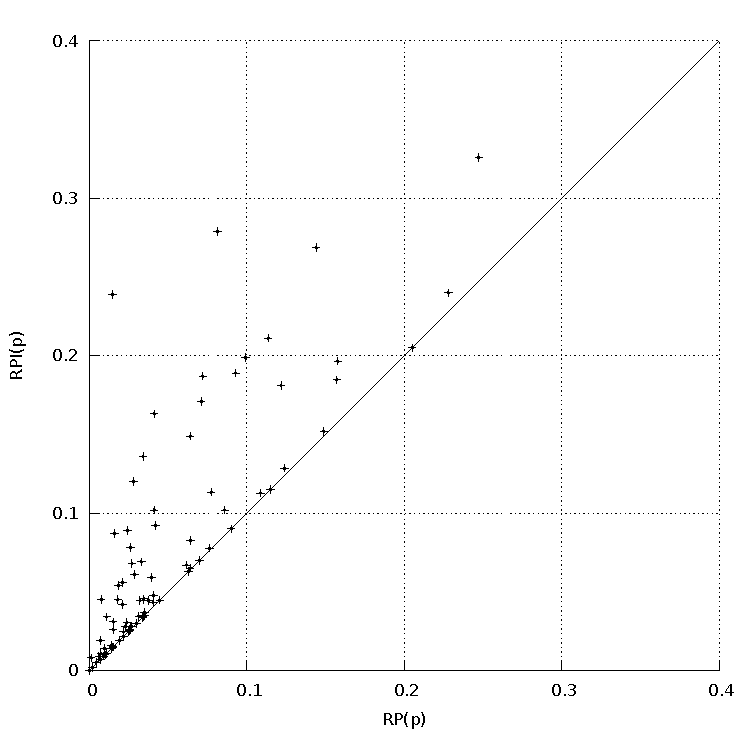
\includegraphics[width=0.45\textwidth]{RPIvsRP.pdf}
  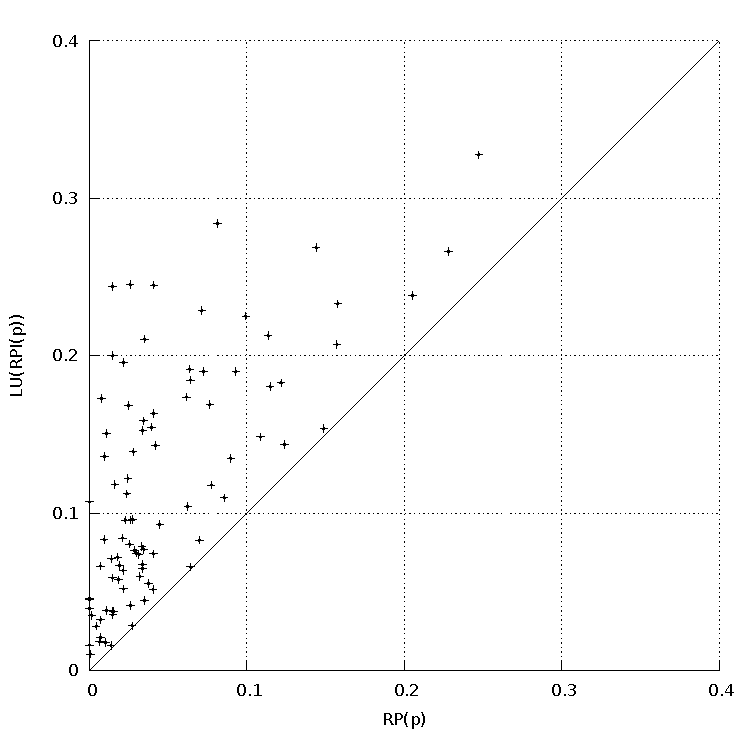
\includegraphics[width=0.45\textwidth]{LURPIvsRP.pdf}
  \caption{Comparing {\RP} and {\RPI}, resp. {\RPI} followed by {\LU}.}
  \label{Fig:RPI-versus-RP}
\end{figure}  

Even though our implementations are just prototypes and the experiments were executed on a modest computer 
(2.8GHz Intel Core 2 Duo processor with only 2GB of RAM (1067MHz DDR3) available for the Java Virtual Machine), 
we were pleased to see that the algorithms presented an acceptable and scalable performance. 
The proofs generated by {\verit} contained up to millions of derived clauses and were up to 100MB big (in the size of the text file) in a 
minimalistic proof format\footnote{This format is closely related to the resolution proof terms used in this 
paper and is quite compact: (1) only the parents of a derived clause must be indicated 
explicitly; % (its literals can be omitted, since they can be recomputed); 
(2) a clause only needs an explicit name/number if it has more than one child.}. 
They included all intermediate clauses that had been learned during the execution of {\verit}, 
even those that were not used to derive the final empty clause. Before applying the compression algorithms, 
we removed these unused clauses, but the pruned proofs were still up to more than half a million clauses long and 
up to about 20MB big. The execution times of all algorithms varied between less
than $100$ miliseconds for the smaller proofs, less than $10$ seconds for the
majority of the much bigger proofs of the SatRace benchmarks, and $7.5$ minutes
in the worst case (for a highly redundant proof with more than half a million
clauses).
% SM: removed the following, which sounds awkward and too defensive to me.
%
%; still acceptable for a non-optimized prototype implementation.

%\begin{figure}[h!]
%\vspace{-20pt}
%\begin{center}
%\leavevmode
%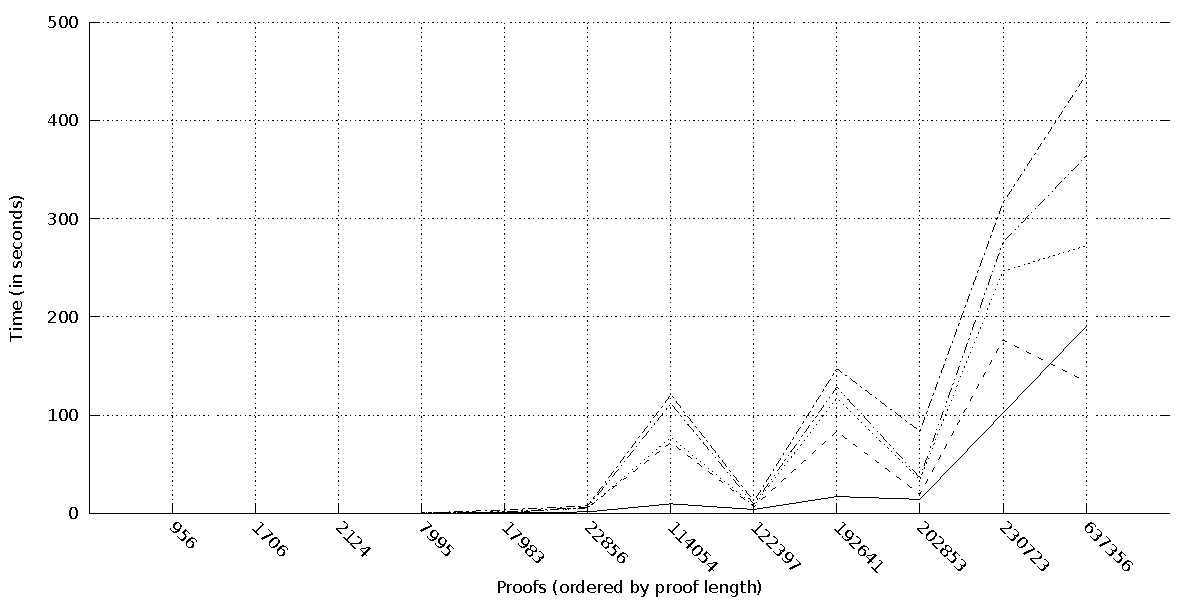
\includegraphics[width=0.8\textwidth]{TimebyProofLength.pdf}
%\end{center}
%%\caption{}
%\label{Fig:TimeSatRace}
%\vspace{-25pt}
%\end{figure}

\begin{figure}[t]
\centerline{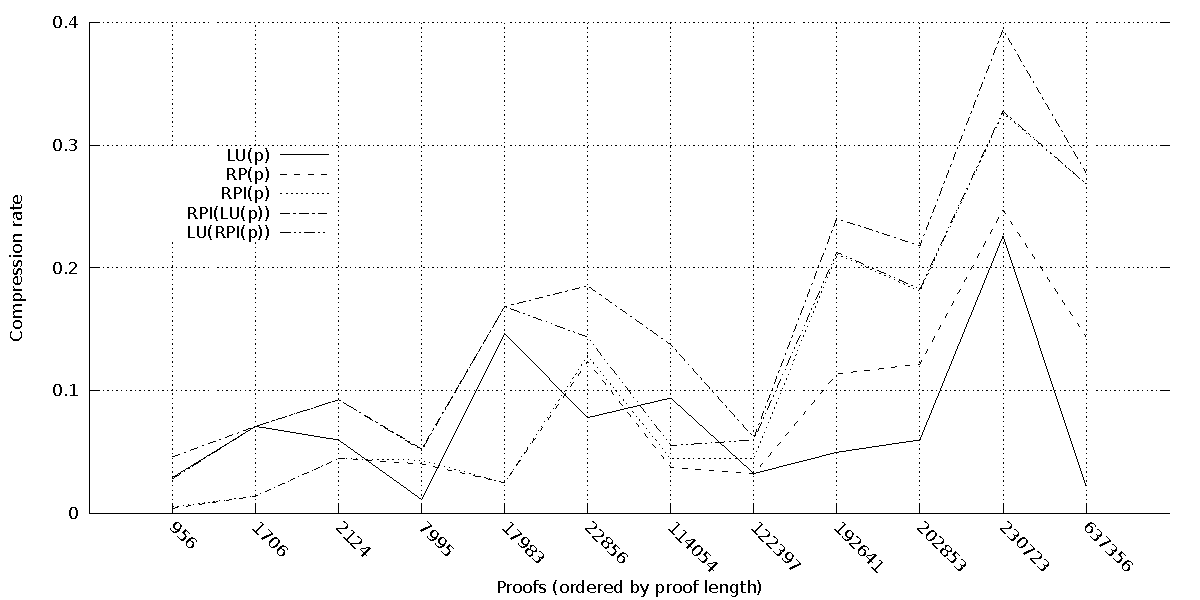
\includegraphics[width=0.8\textwidth]{RatebyProofLength.pdf}}
\centerline{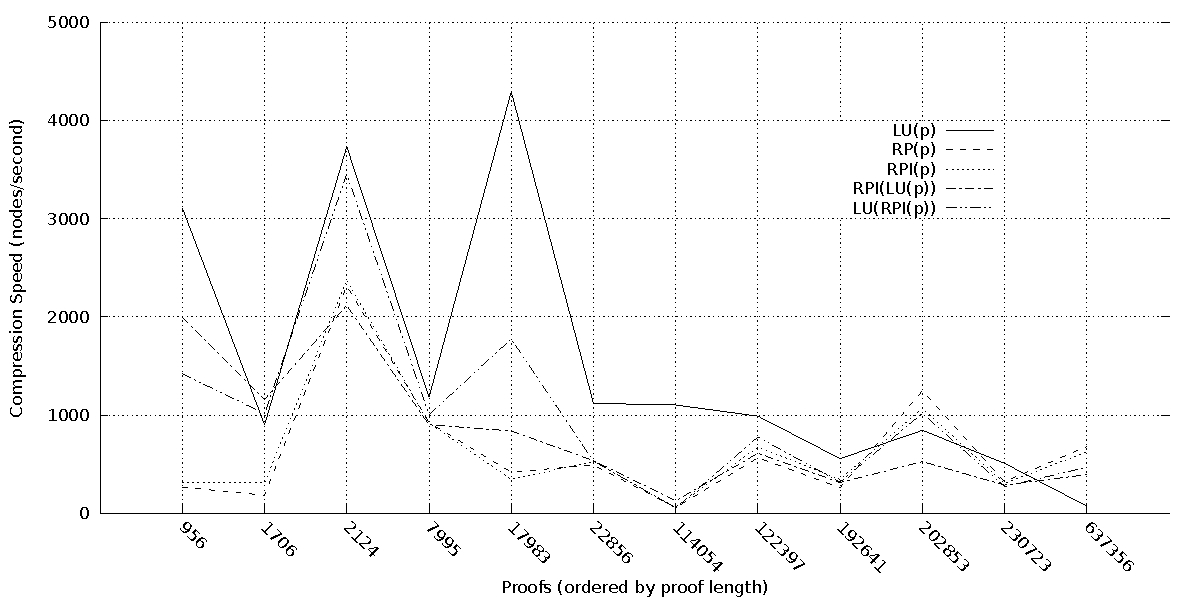
\includegraphics[width=0.8\textwidth]{SpeedbyProofLength.pdf}}
\caption{Compression and compression speed for the SatRace examples.}
\label{Fig:CompressionSatRace}
\end{figure}

Figure~\ref{Fig:CompressionSatRace} shows the compression (top) and compression
speed (bottom) for the examples from the SatRace. The top figure
suggests a trend where longer proofs are more redundant and allow for more
compression. This might be due to the fact that the SAT solver backtracks and
restarts more often for harder problems that generate longer proofs.

The bottom figure shows that compression speeds of the {\RPI} and {\RP}
algorithms are very similar, although {\RPI} took significantly more time than
{\RP} for some examples.
In cases where the compression rates are comparable, the execution times are
similar as well. When {\RPI} took more time than {\RP}, it achieved
correspondingly better compression. This indicates that computing the
intersections is worthwhile in practice. Finally, note that {\LU} is usually the fastest algorithm in terms of compression speed.
 
% \begin{figure}[t]
% \caption{Compression achieved with {\RPI} followed by {\LU} or in reverse order.}
% \label{Fig:ComparingTwoCombinations}
% \end{figure}

\smallskip

\centerline{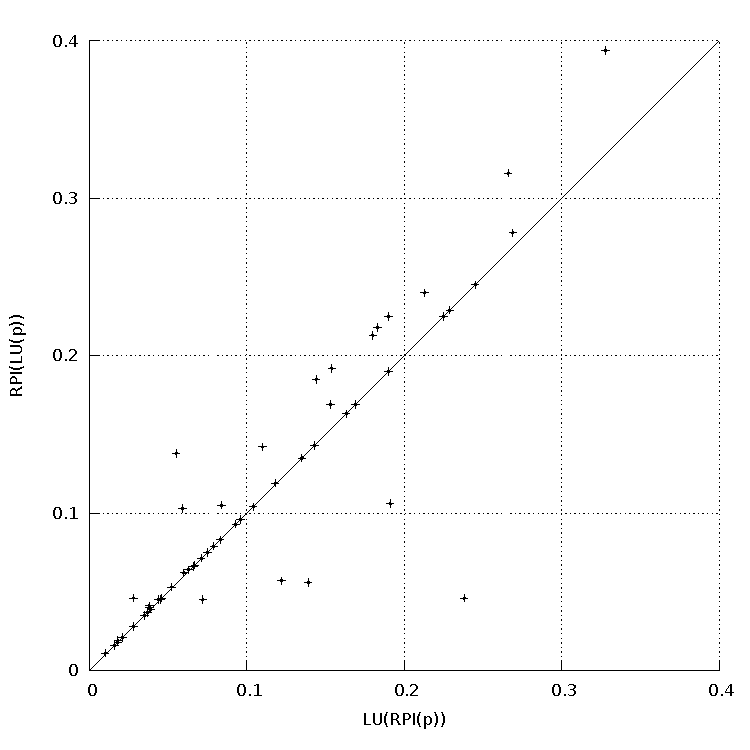
\includegraphics[width=0.45\textwidth]{RPILUvsLURPI.pdf}}

\smallskip

The compression achieved by applying both {\LU} and {\RPI} is usually less than
the sum of the compressions achieved by each algorithm alone. This is so because
certain redundancies are eliminated by both algorithms. Moreover, the scatter plot
above shows that the order in which {\LU} and {\RPI} are applied matters. 

%% SM: removed the following because it is not particularly illuminating.
%%
% Since
% {\LU} and {\RPI} eliminate redundancies in different ways, choosing which one to
% apply first determines how many nodes and edges are removed from the proof.



\section{Related Work and Ideas for Future Work}
\label{sec:related}

One of the kinds of local redundancy was considered in our previous
work~\cite{FontaineMerzPaleo2010Exploring-and-Exploiting-Algebraic-and-Graphical-Properties-of-Resolution},
where we also proposed \emph{resolution hypergraphs} as a possible non-linear
notation for resolution proofs, making it easier to identify and address
non-local redundancies. Although in principle more general than the techniques
described here, they do not scale to large proofs, because resolution
hypergraphs can be exponentially larger than the proofs they represent.


The same kind of local redundancy was also mentioned by Simone et al.~\cite{SimoneBrutomessoSarygina2010An-Efficient-and-Flexible-Approach-to-Resolution-Proof-Reduction}, 
as the local proof rewriting rule $A1'$. They address global redundancies by having another local proof 
rewriting rule ($A2$) that performs inference permutations when possible. 
As we have argued before, this approach is inherently inefficient, since too many permutations would have to be considered in order to eliminate all global redundancies. 
They also consider other interesting local proof rewriting rules that eliminate redundancies not considered in this paper. It would be worthwhile to generalize these other kinds of local redundancy by defining 
their global counterparts too; it might then be possible to adapt the global techniques described in this paper 
to these other kinds of redundancy.

Besides {\RP}, Bar-Ilan et al.~\cite{Bar-IlanFuhrmannHooryShachamStrichman2009Linear-time-reductions-of-resolution-proofs} also defined the \texttt{RecycleUnits} algorithm, which replaces one of the parents of a resolvent with a resolved literal $\ell$ by a unit clause containing $\ell$, if such a unit clause exists somewhere else in the proof. Although this algorithm eliminates some kinds of redundancy, it generates redundancies of the kind handled by {\LU}. Therefore it would be helpful to always execute {\LU} after \texttt{RecycleUnits}, or to combine both algorithms more tightly: instead of replacing a parent by the unit, the resolvent can be replaced by the other parent, and the unit can be queued to be reinserted at the bottom of the proof.

Cotton~\cite{Cotton2010Two-Techniques-for-Minimizing-Resolution-Proofs} proposes
to split a refutation $\psi$ into a proof $\psi_{p}$ of the unit clause containing the atom $p$ and a proof $\psi_{\neg p}$ of unit clause containing the literal $\neg p$. This is done by deleting one of the parents of every resolvent with pivot $p$. A new refutation $\psi'$, possibly shorter than $\psi$, is then obtained by resolving $\psi_{p}$ and $\psi_{\neg p}$. Since in $\psi'$ there is now only one resolvent with pivot $p$, all potential redundancies with pivot $p$ are removed with this splitting technique. Consequently, in principle this splitting technique could subsume all other techniques previously described, including the ones in this paper. However, since not all potential redundancies are actual redundancies, $\psi'$ might actually be longer than $\psi$. This problem is atenuated by heuristically choosing a promising literal $p$ to split, and iterating until the next proof $\psi'$ becomes longer than the current proof $\psi$. The techniques that globally identify precisely which potential redundancies are actual redundancies, such as those presented in \cite{Bar-IlanFuhrmannHooryShachamStrichman2009Linear-time-reductions-of-resolution-proofs} and here should scale better, since they do not need to iterate an undefined number of times and fix the proof after every iteration.

While this paper focused on regularization of proofs, trying to compress proofs by introducing 
irregularities is also an interesting possibility to be investigated in future work, 
since exponential compression might be achieved in the best cases.
%\cite{Amjad2006Compressing-propositional-refutations}

%\cite{Amjad2008Data-Compression-for-Proof-Replay}

\section{Conclusions}

The use of proof contexts makes for a clear transition from local to global
transformations of proofs, and in particular helped us generalize certain kinds
of local redundancies to global ones. In this way, we designed two algorithms
that eliminate these global redundancies more efficiently than previous ones.
Our experiments seem to indicate that we can expect reductions of around 20\%
for large proofs, beyond what is possible just by pruning irrelevant inferences.
Since these reductions essentially come for free and proof checking can be
costly (for example when it is performed by the trusted kernel of an interactive
proof assistant or when it has to be repeated many times by different proof
consumers such as in a PCC scenario), we believe that it is
worthwhile to implement our techniques when proof size matters.

\bibliographystyle{abbrv}
\bibliography{Bibliography}

\end{document}
